\section{Motivation}
\begin{frame}{Why spikes ?}{\insertsection}
    \begin{itemize}
        \item An approach from \textprim{Analog-to-Digital conversion} and \textprim{digital communications}
        \item Spiking mechanism as a conversion from analog ( continuous time, continuous space) to digital (discrete time and/or discrete space)
        \item How can we exploit this mechanism to design digital hardware ?
    \end{itemize}
    \begin{figure}
        \centering
        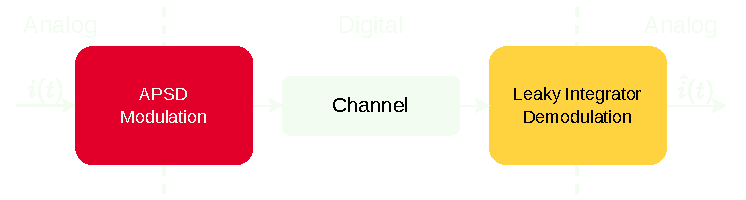
\includegraphics[width=.8\columnwidth]{Figures/overview.pdf}
    \end{figure}
\end{frame}

\section{Spike Response Model}
\subsection{Neuron Model}
\begin{frame}{Spike Response Model $0^{th}$ order \cite{gerstner_spiking_2002}}{\insertsection ~- \insertsubsection}
    \begin{columns}
        \column{0.35\paperwidth}
        \begin{figure}
            \centering
            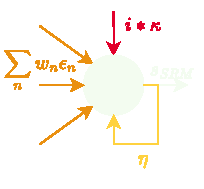
\includegraphics[width=.8\columnwidth]{Figures/srm_neuron.pdf}
        \end{figure}
        \vspace{-0.7cm}
        \begin{itemize}
            \item $\kappa$ : input response
            \item $\eta$ : output response
            \item $\epsilon$ : presynaptic spike response
        \end{itemize}

        \column{0.6\paperwidth}
        \begin{align*}
            v_{SRM}(t) = \textprim{i(t) * \kappa (t)} &+ \\
            \textter{\sum_{m=1}^{M_{SRM}} \eta(t-T_m^{SRM})} &+ \\
            \textbis{\sum_{n=1}^{N} w_n \sum_{m_n=1}^{M_n} \epsilon_n (t-T^{n}_{m_n})}\\
            s_{SRM}(t) \triangleq \sum_{m=1}^{M_{SRM}} \delta (t-T_m^{SRM})
        \end{align*}
    \end{columns}
\end{frame}

\begin{frame}{Alternative Form}{\insertsection ~- \insertsubsection}
    \begin{columns}
    \column{0.45\paperwidth}
    \begin{align*}
        y_{SRM}(t) &\triangleq i(t) * \kappa (t)\\
        \hat{y}_{SRM,L}(t) &\triangleq - \sum_{m=1}^{M_{SRM}} \eta(t-T_m^{SRM})\\
        &= -\eta(t) * s_{SRM}(t)\\
        v_{SRM}(t) &= y_{SRM}(t) - \hat{y}_{SRM,L}(t)
    \end{align*}

    \column{0.5\paperwidth}
    \begin{itemize}
        \item $y_{SRM}(t)$ : input current response filter
        \item $\hat{y}_{SRM,L}(t)$ : unsmoothed reconstruction estimate of $y_{SRM}(t)$
    \end{itemize}

    \begin{box_prim}{Remark}
        \begin{itemize}
            \item Tracking error is bounded by $v_t$
        \end{itemize}
    \end{box_prim}

    \end{columns}
\end{frame}

\begin{frame}{Filter Building Block}{\insertsection ~- \insertsubsection}
    \begin{figure}
        \centering
        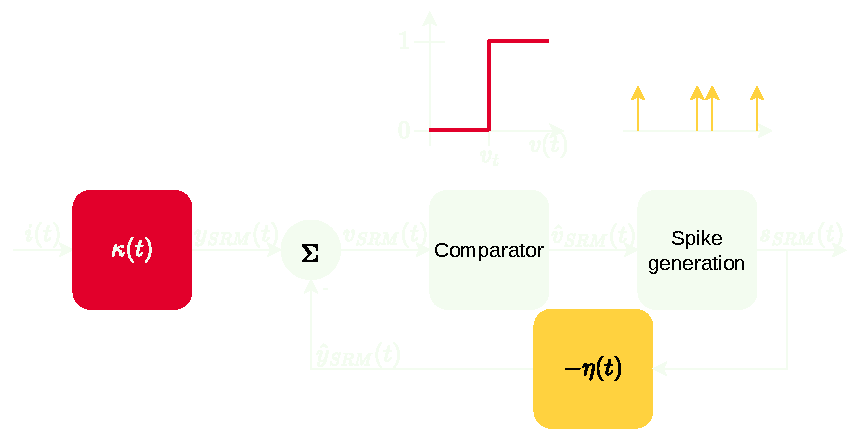
\includegraphics[width=.9\columnwidth]{Figures/srm_filter.pdf}
    \end{figure}
\end{frame}

\begin{frame}{Signals}{\insertsection ~- \insertsubsection}
    \begin{columns}
    \column{0.45\paperwidth}
    \begin{figure}
        \centering
        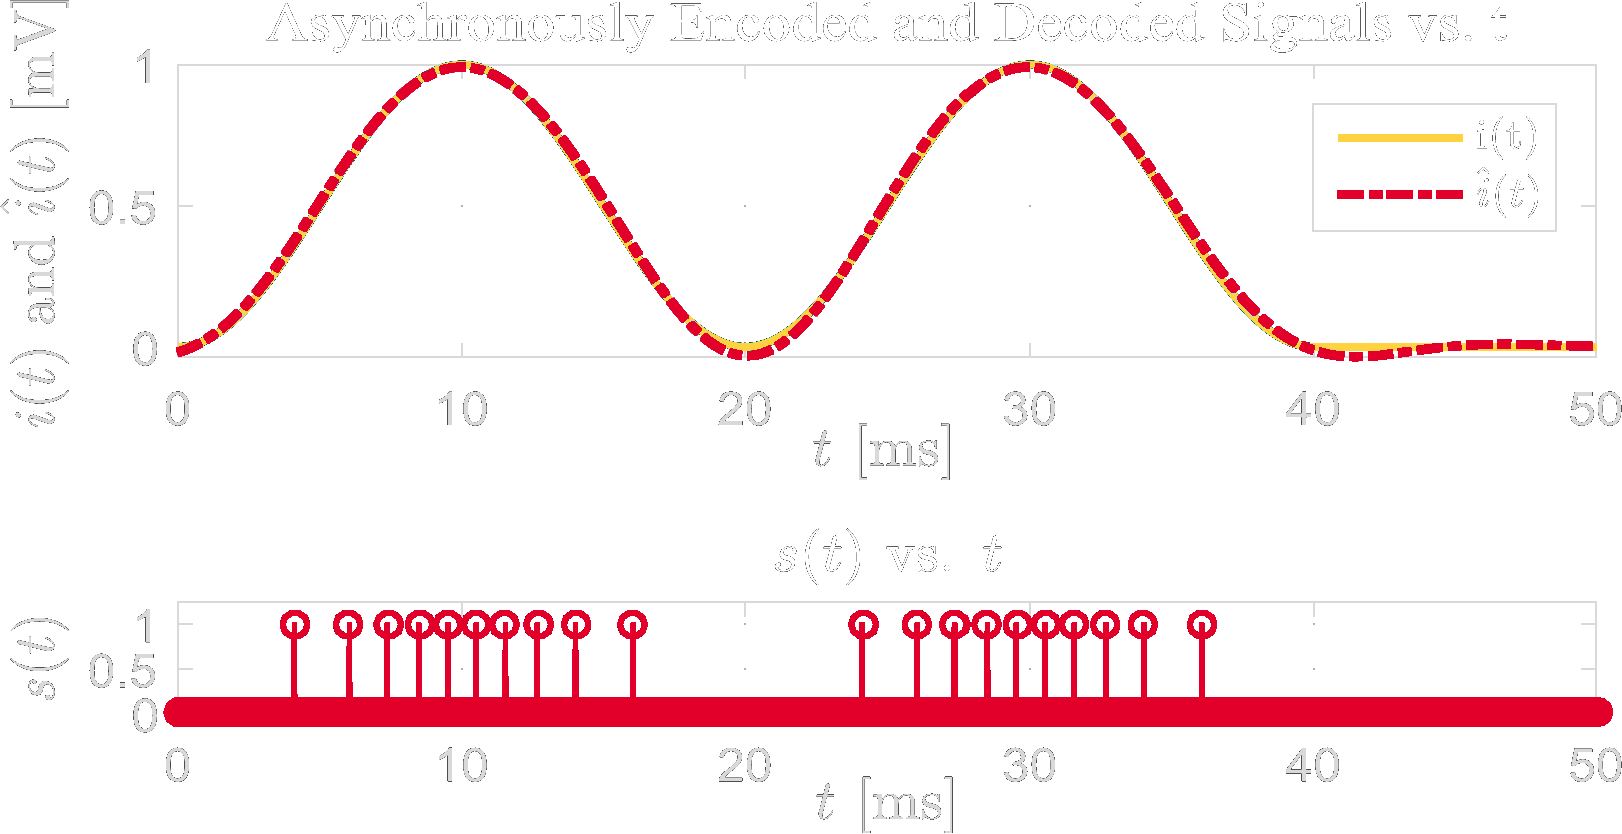
\includegraphics[scale=0.5]{Figures/signal_io.png}
    \end{figure}

    \column{0.45\paperwidth}
    \begin{figure}
        \centering
        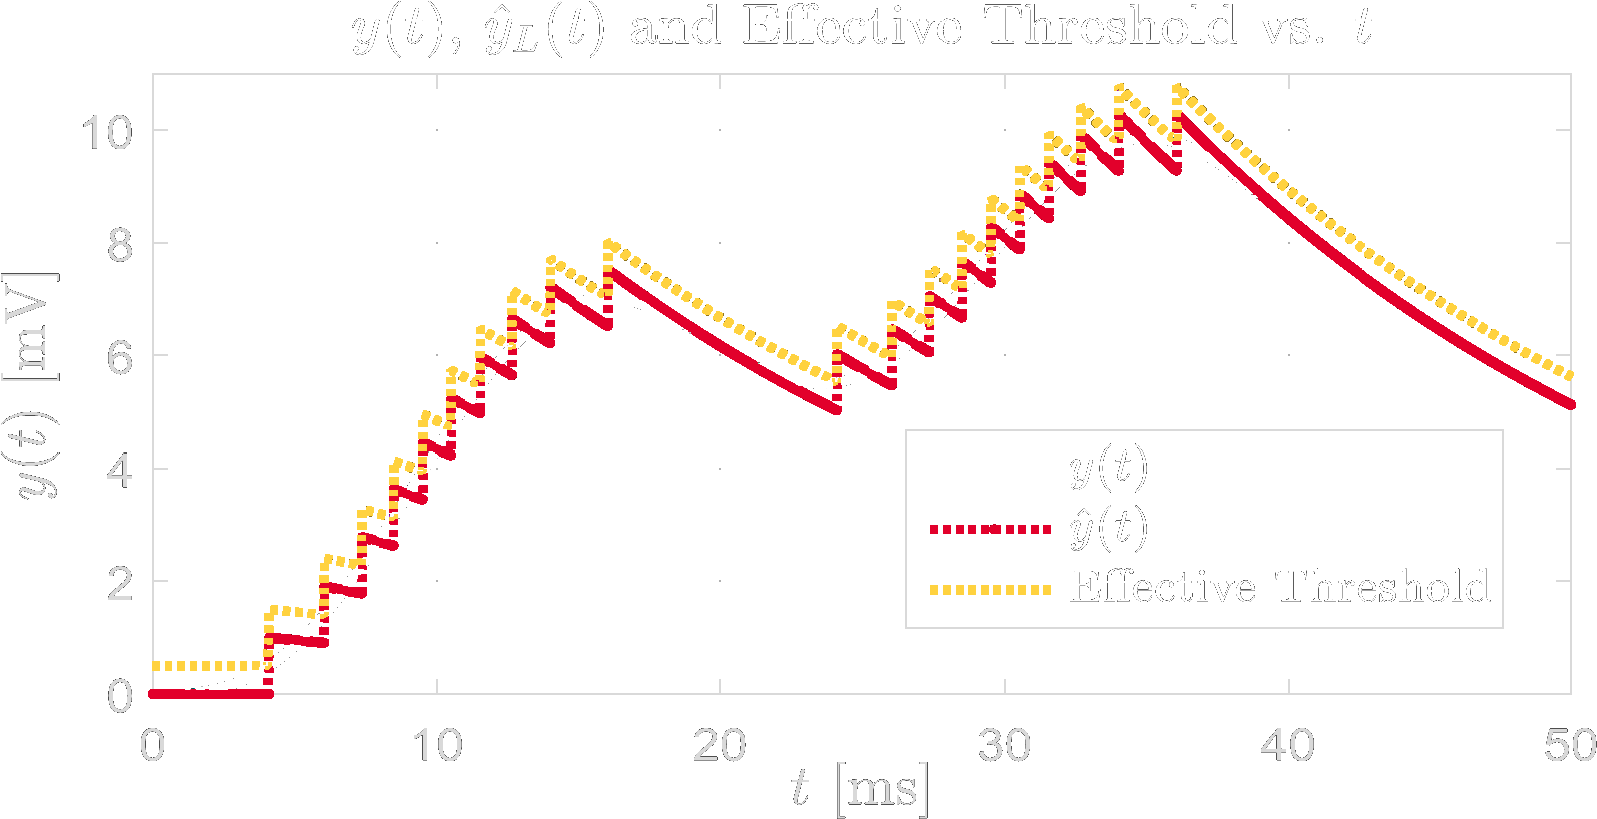
\includegraphics[scale=0.5]{Figures/signal_y.png}
    \end{figure}
    \begin{figure}
        \centering
        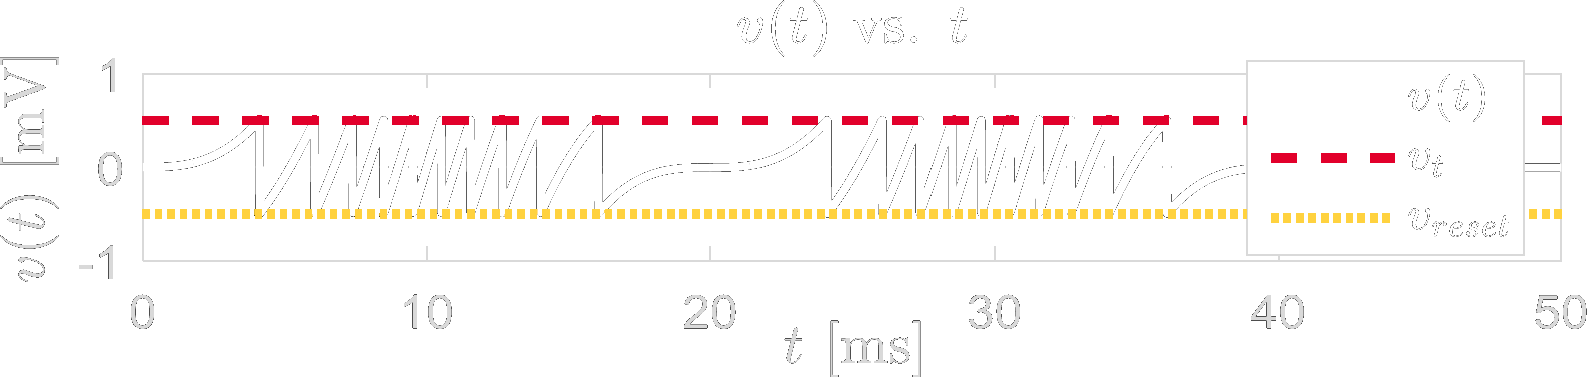
\includegraphics[scale=0.5]{Figures/signal_v.png}
    \end{figure}

    \end{columns}
\end{frame}


\section{Sigma-Delta Modulation}
\subsection{Canonical Form}
\begin{frame}{Where is the integral ?}{\insertsection ~- \insertsubsection}
    \begin{figure}
        \centering
        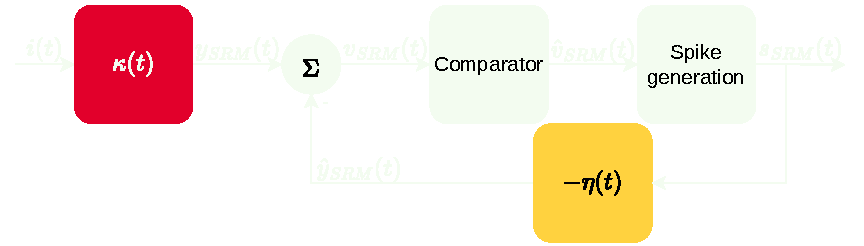
\includegraphics[width=.9\columnwidth]{Figures/srm_filter_simp.pdf}
    \end{figure}
\end{frame}

\begin{frame}{Special case}{\insertsection ~- \insertsubsection}
    \begin{columns}
    \column{0.4\paperwidth}
    \only<1->{
    \begin{figure}
        \centering
        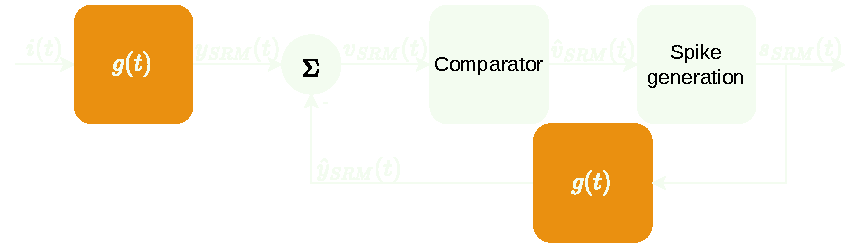
\includegraphics[width=\columnwidth]{Figures/srm_filter_spec.pdf}
    \end{figure}
    }
    \only<2->{
    \begin{figure}
        \centering
        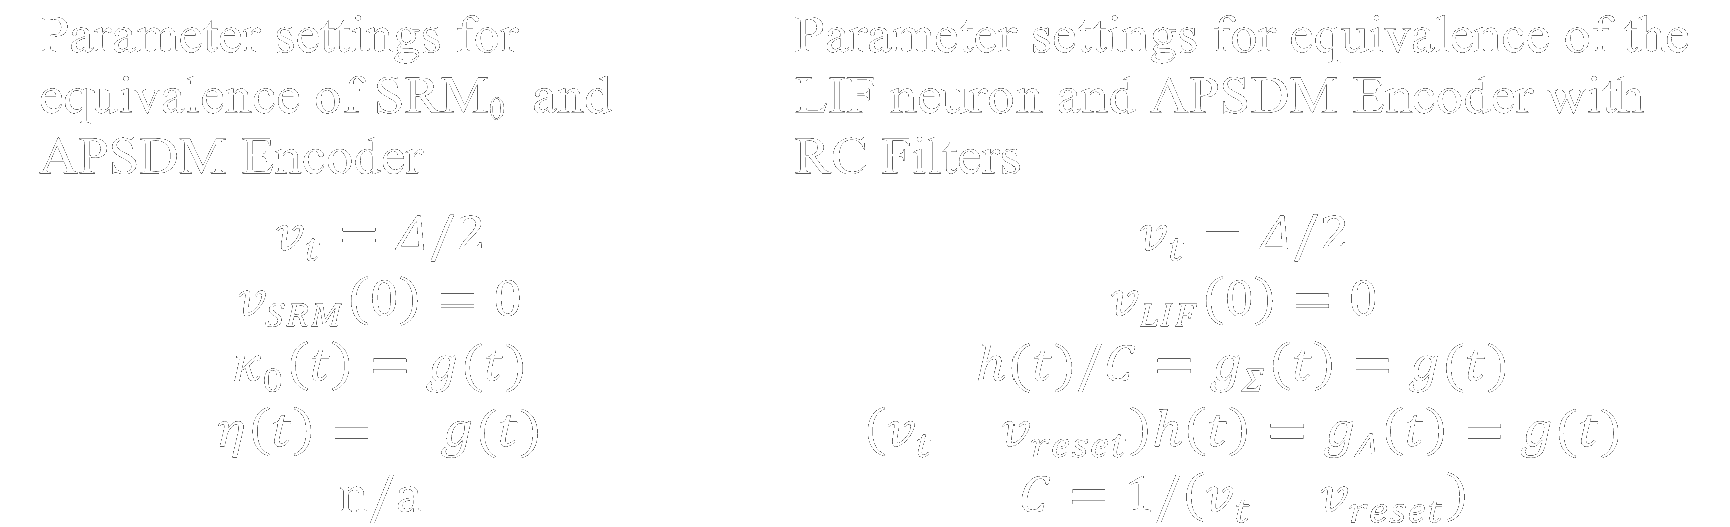
\includegraphics[width=\columnwidth]{Figures/condition.png}
    \end{figure}
    }


    \column{0.55\paperwidth}
    \only<2->{
    \begin{figure}
        \centering
        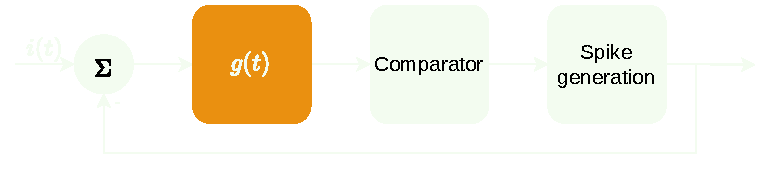
\includegraphics[width=\columnwidth]{Figures/srm_filter_spec_simp.pdf}
    \end{figure}
    }
    \only<3->{
    \begin{figure}
        \centering
        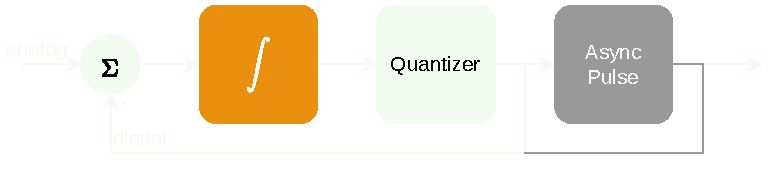
\includegraphics[width=\columnwidth]{Figures/sdm_canon.pdf}
    \end{figure}
    }

    \end{columns}
\end{frame}

\section{Demodulation}
\begin{frame}{\insertsection}

    \only<1>{
    \begin{figure}
        \centering
        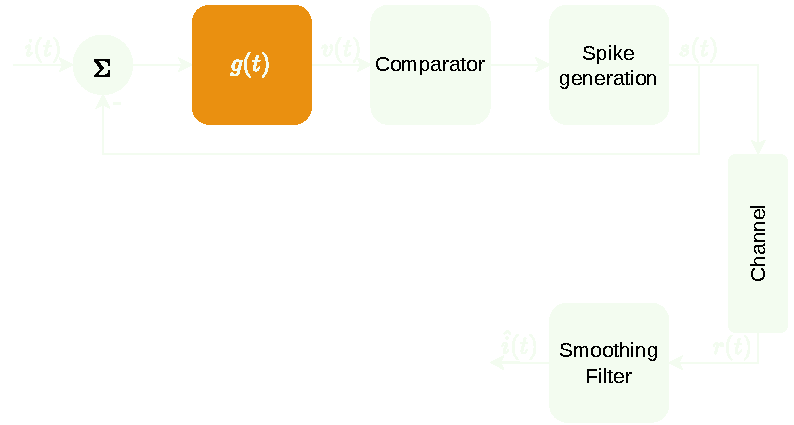
\includegraphics[width=.9\columnwidth]{Figures/sender_receiver.pdf}
    \end{figure}
    }
    \only<2>{
    \begin{figure}
        \centering
        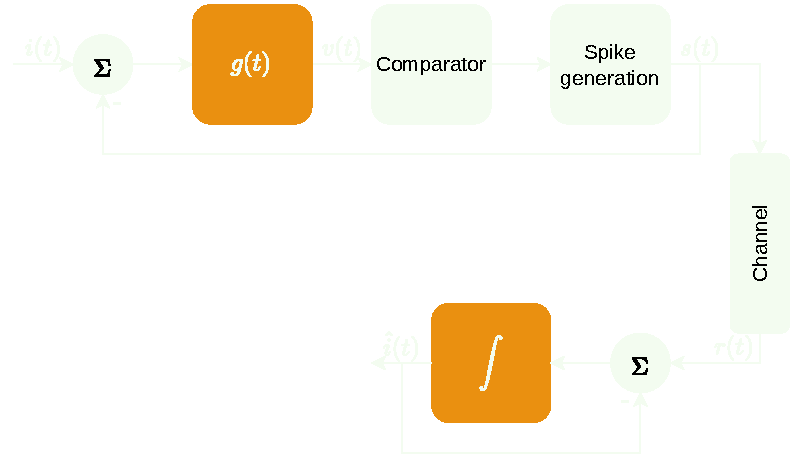
\includegraphics[width=.9\columnwidth]{Figures/sender_receiver_LI.pdf}
    \end{figure}
    }
\end{frame}

\section{Conclusion}
\begin{frame}{Summary}{\insertsection}
    \begin{figure}
        \centering
        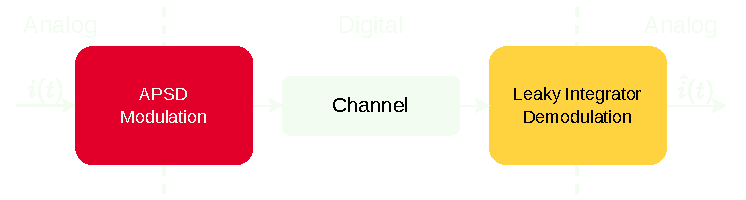
\includegraphics[width=.8\columnwidth]{Figures/overview.pdf}
    \end{figure}
    \begin{itemize}
        \item Formulation as the difference of an input response filter and its approximation
        \begin{itemize}
            \item Approximation error and spike frequency both depend on the threshold
        \end{itemize}
        \item Can be mapped to asynchronous pulse sigma-delta modulation
        \item Demodulation can be done by a low pass filter such as a Leaky Integrator
    \end{itemize}
\end{frame}

\begin{frame}{Perspectives}{\insertsection}
    \begin{itemize}
        \item APSDM is a simple case (unipolar, one threshold) but it can be extended (e.g. bipolar send-on-delta)
        \item What does it mean for processing with neurons ? \item How do we relate this with numerical solvers ?
        \item How can we exploit this structure to produce neuromorphic HW ?
        \item How biologically plausible is all of that ?
        \begin{itemize}
            \item Neuronal Spike Generation Mechanism as an Oversampling, Noise-shaping A-to-D Converter - Chklovskii & Soudry \cite{chklovskii_neuronal_2012}
        \end{itemize}
    \end{itemize}

    Further reading : \cite{schindler_linear_1974}, \cite{kikkert_asynchronous_1975}
\end{frame}